\documentclass[10pt,a4paper]{article}
\usepackage{graphicx}
\usepackage[a4paper, total={6in, 9in}]{geometry}
\graphicspath{ {/} }
\usepackage{amsmath}
\usepackage{algorithm}
\usepackage[noend]{algpseudocode}
\usepackage{enumerate}
\usepackage{float}
\usepackage{amssymb}

\makeatletter
\def\BState{\State\hskip-\ALG@thistlm}
\makeatother

\begin{document}
	
	\section*{Problem 1}

	In this problem we were asked to use a genetic algorithm to determine a satisfiable solution for various 3-CNF statements. All of these 3-CNF statements used as benchmarks were satisfiable, our benchmarks only determine if a satisfiable solution can be found with certain time limits. Each statement was contained in its own file. We tested our algorithm on 100 different benchmarks (files) for 20, 50, 75, and 100 variable 3-CNF problems. The algorithm was allowed to run three times for each benchmark each time with a 250ms, 500ms, and 750ms time limit respectively. If an algorithm ran to its alotted time limit it was said to be a failure and was terminated.

	\begin{center}
		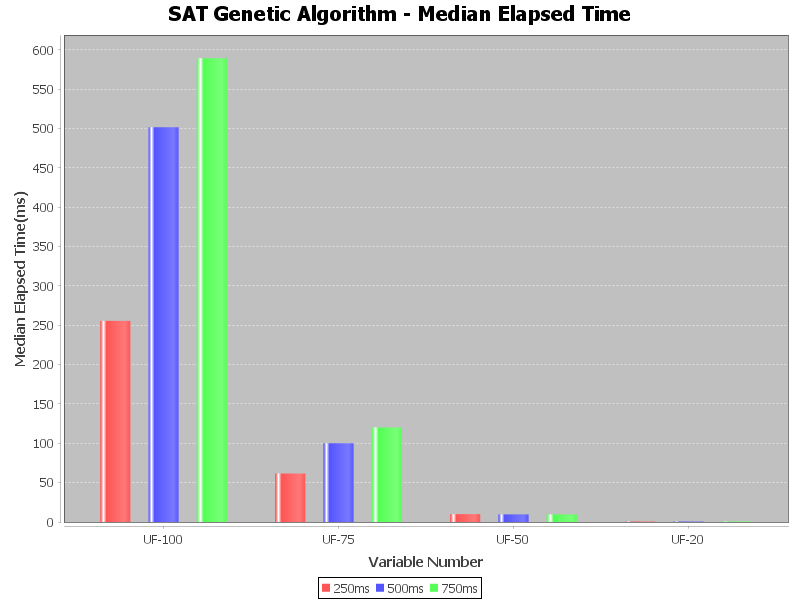
\includegraphics[scale=0.35]{median_time}
	\end{center}
	
	\textbf{Median Elapsed Time:} Above is a graph displaying the results of our benchmark evaluations in terms of the median elapsed time. The most interesting result here occured in our UF-100 tests. For the 250ms time limit and 500ms time limit tests the average median time was 250ms and 500ms respectively. Clearly, this means that none were allowed to run to completion and failed to find a satisfiable solution in their time limits. With a 750ms time alottment however, the average runtime was about 580ms implying many, but not all, ran to completion.
	
	As a trend, the fewer variables a problem had, the less runtime it required. 20 variable problems required median runtimes of less than 5ms on average. 50 variable problems required median runtimes of less than 25ms on average. Based on the results of our benchmark evaluations it seems as though the trend may be that as the number of variables increases the median runtime increases exponentially. This is hard to see in the UF-100 column as the times were explicitly limited to 250 and 500ms and thus solution to completion cannot accurately be described. More benchmark evaluations would be required to prove definitively that this is the relationhip.
	
	\begin{center}
		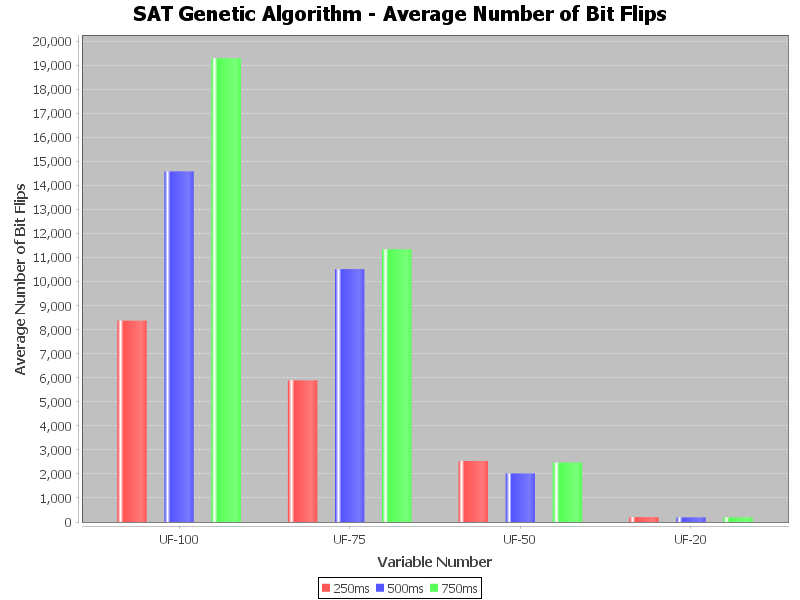
\includegraphics[scale=0.35]{average_bitflips}
	\end{center}
	
	\textbf{Average Number of Bit Flips:} Above is the average number of bit flips the algorithm used during the flip heuristic segment of its code for each of our benchmarks. Clearly, the more variables a problem had, the more bitflips it required during execution of the algorithm. 
	
	For UF-100 and UF-75, tests with lower time limits yielded on average less bitflips. This is due to the fact that many of these runs did not run until they found a satisfiable state, but were instead cut off by their time limites. This effect is noticable when compared with our UF-50 and UF-20 runs which did not have a correlation between time limit and average bitflips. 
	
	In general, as the number of variables in the problem increased the number of bitflips that were required to find a satisfiable solution (or until time ran out) greatly increased.
	
	\begin{center}
		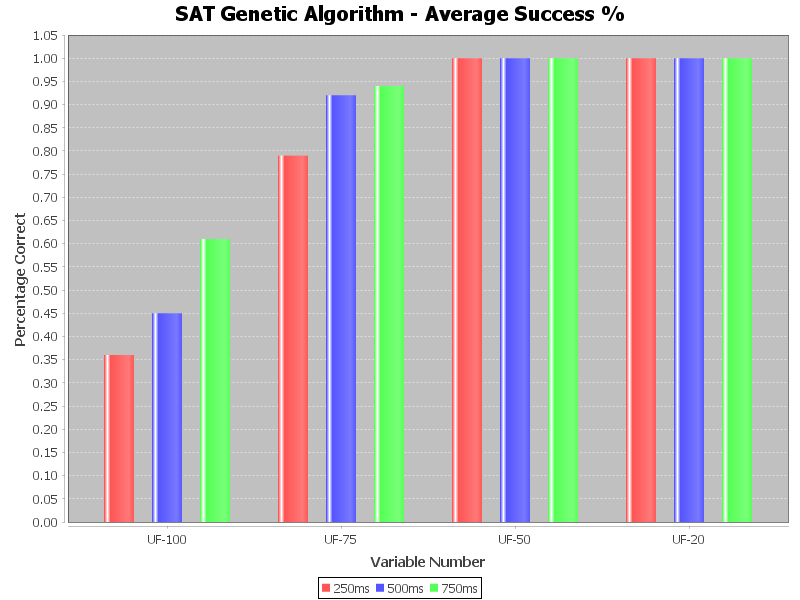
\includegraphics[scale=0.35]{average_success}
	\end{center}
	
	\textbf{Success Percentage:} Above is a chart displaying the percentage across all of our benchmarks that a satisfiable solution for the 3-CNF problem was found.For our UF-20 and UF-50 benchmark evaluations, for all given time limits (250ms, 500ms, and 750ms) every benchmarks that was ran was able to find a satisfiable solution.
	
	As the number of variables in the problem increased however we see that more runs began to reach their time limits. For our UF-75 tests, more than 90\% of benchmark evaluations were able to find a satisfiable solution with both a 750ms and 500ms time limit. However, decreasing the time limit to 250ms we began to see our first real drop in percentage successful down to 78\%.
	
	The success rate was worse for our 100 variable benchmarks tests. Naturally, as we reduced the alotted time, less of these runs were able to find a satisfiable solution. Our worst success rate was for UF-100 with an alotted time of 250ms. Here, only 36\% of all runs managed to find a satisfiable solution before the time limit. Clearly the results of this section show that as the number of variables in the 3-CNF problem increases, the more time is necessary for the algorithm to find a satisfiable solution.
	
	\section*{Problem 2}
	
	\begin{enumerate}[A.]
		\item
		\begin{center}
			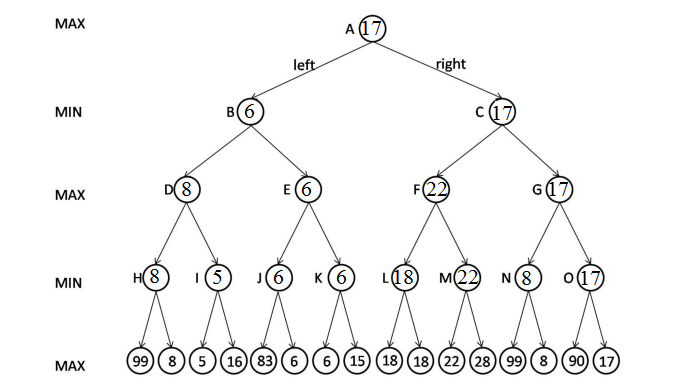
\includegraphics[scale=0.5]{Minimax}
		\end{center}
		\item
		\begin{center}
			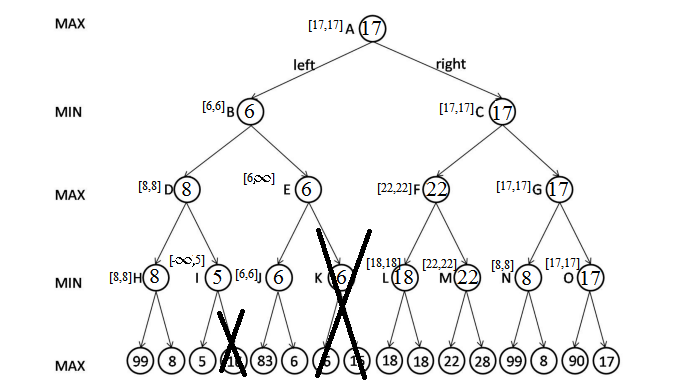
\includegraphics[scale=0.5]{Pruning}
		\end{center}
		
		We cut off the subtree at node K since node B is a MIN and will only accept a value less than 8 we know that we wont get a value greater than 6 down said subtree. The same also occurs below node I. The terminal node 15 is pruned because node D will accept any number greater than 8 however, node I is a MIN and the left terminal node being 5 allows us to denote that the right terminal node cannot be less than 5.
		
		\item 
		The max player will choose 17 at the root state by using the exhaustive Minimax Algorithm. The same result will occur when using alpha-beta pruning
		and the max player will again choose 17. The most optimal move is guaranteed using either the exhaustive Minimax algorithm or the alpha-beta pruning algorithm. This is accomplished by alpha-beta pruning ignoring subtrees that are irrelevant while exhaustive Minimax algorithm checks every node regardless of relevance. The outcome is the same however, since alpha-beta pruning ignores irrelevant subtrees it is more efficient.
		
		\item
		
		In this version of minimax we are using alpha-beta pruning as well as guiding heuristic values. The heuristic values that were given in the problem  were as follows: $h(D)=9$ $h(E)=7$ $h(F)=24$ $h(G)=16$. 
		
		Because the heuristic value for node E is lower than the heuristic value for node D, and since their parent node B is a MIN, the subtrees with root D and root E will be swapped. This is because, based on the heuristic values, the algorithm would want to search the subtree of node E first, since B is a minimizer and would would choose the minimal value, it is more likely that we can eliminate nodes that we need to search if we search this subtree first.
		
		The same is true for nodes F ang G. Node G has a lower heuristic value and since their parent node C is a MIN node, it will choose the minimal value of the two children nodes. Since the heuristic is informing us that G is most likely the node with the minimal value, we will expand G first to see if there are any nodes we can possibly eliminate from our search process.
		
		Node A is a MAX. Based on the information provided by the heuristic we can determine which subtree, B or C, would be better to search first. Since B is a MIN, and we know that $h(D)=9$ and $h(E)=7$ we can assume that node B would choose node E. The same logic can be applied to see that node C will choose node G. Now we know that based on the heuristic node B has a value of 7 and node C has a value of 16. Since A is a MAX it should expand node C first, so B and C are swapped.
		
		The specified swaps are shown below:
		
		\begin{center}
			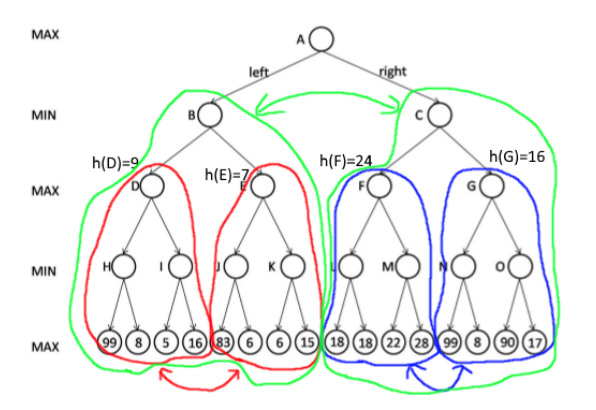
\includegraphics[scale=0.5]{alphabeta_swaps}
		\end{center}
		
		After these swaps are made the minimax algorithm with alpha-beta pruning will run in its normal operation and find that the following nodes will not need to be expanded:
		
		\begin{center}
			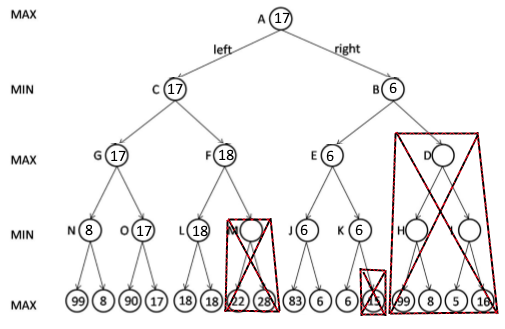
\includegraphics[scale=0.5]{alphabeta_elim2}
		\end{center}
		
		Clearly, using the information provided by the heuristic values, the minimax algorithm using alpha-beta pruning will find than it can eliminate more nodes that its uninformed counterpart and still find an optimal solution.
		
		\item
		
		Consider a variation where the MIN player will choose either the left or right child state as its move with a 0.50 probability. Here, the MAX player is uncertain what node to choose because it cannot predict the choice of the MIN player based on the minimum value available to it (as in a typical minimax search tree). However, the MAX player can choose a value in the search tree based on the expected value of the MIN players choice.
		
		For example, if a MIN player has available to it a node with a utility value of 5 and a node with a utility value of 15, based on this problem we know that it will choose 5 with probability 0.50 and 15 with probability 0.50. Therefore we can say the expected value of the MIN players choice is 10. For each MIN node, we can say that its expected value is $0.50*\textit{value of left child} + 0.50*\textit{value of right child}$. The MAX player can then maximize its choice by selecting the MIN node with the higher expected value, and in this way we utilize all of the information available to our MAX player to optimize his choice based on the randomness of the MIN player.
		
		\begin{center}
			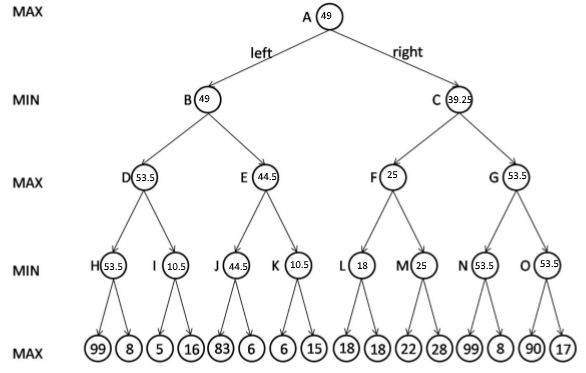
\includegraphics[scale=0.75]{random_minimax}
		\end{center}
		
		Above is a visualization of the described algorithm where the MIN player stores in its node its expected value from choosing from its two children each with 0.50 probability. The MAX player will then choose the MIN node with the higher expected value.
		
	\end{enumerate}


	\section*{Problem 3}

	
	\begin{enumerate}[A.]

		\item
		
		\textbf{Variables:} Defined as $n_{i,j}$ where $i \in \text{\{set of all row numbers\}}$ and $j \in \text{\{set of all column numbers\}}$ for each cell $n$ on the board. Essentially, each square on the sudoku board will be a variable, for a total of 81 variables.
		
		\textbf{Domain:} Defined as the set of possible values in sudoku. Here, this set is defined as $\{ 1, 2, ..., 9 \}$
		
		\textbf{Constraints:}
		
		\begin{enumerate}[1.]
			\item All variables in any row must be assigned distinct values.
			\item All variables in any column must be assigned distinct values.
			\item All variables in any 3x3 region must be assigned distinct values.
			\item The assignments given to variables in the start state cannot be changed.
		\end{enumerate}
		
		\item
		
		\textbf{Start State:} The start state is a given board that has variables assigned with certain values. These values are the basis for the constraints for the rest of the problem and may not be changed. Below is an example start state.
		
		\begin{center}
			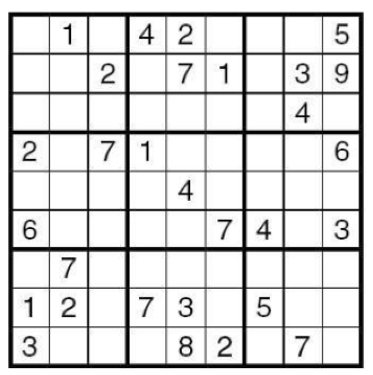
\includegraphics[scale=0.4]{sudoku_startstate}
		\end{center}
		
		\textbf{Successor Function:}  
		
		\begin{enumerate}[1.]
			\item Select a random unassigned variable 
			\item Assign a value to this variable that does not violate any constraints
			\item The resulting state is the successor
		\end{enumerate}
		
		\textbf{Goal Test:} A state is considered to a valid goal state if it is both consistent and complete.
		
		\textbf{Path Cost Function:} The path cost from any one state to its successor state will be 1.
		
		\item 

		Sudoku problems that are easy compared to ones that are hard can be determined based on the relative usefulness of applying the minimum remaining values heuristic to their search states. 
		
		Consider a Sudoku board for which there are an equal number of remaining values for each variable based on their constraints. Here, the heuristic will not be of much use to us since it will not help us narrow our search and we will have to backtrack from many more states to find a satisfiable goal state than if we were faced with an easier Sudoku board.
		
		An easier Sudoku board can be defined as one for which there is a varied range of minimum remaining values for each variable. This will be an easier game because the minimum remaining values heuristic will direct us to expand states with the least minimum remaining values first. Since the distribution of minimum remaining values for an easy board is more varied, there will always be a good estimate of what state to expand next and this will lead us more directly to the goal state.

		\item Pseudocode for Local Search

		\begin{algorithm}[H]
			\caption{Sudoku Local Search Algorithm}\label{euclid}
			\begin{algorithmic}[1]
				\Procedure{SudokuSolver}{$\text{Board}$ $\textit{board}$}
				\State $\textit{board} \gets \text{randomizeCompleteState(\textit{board})}$
				\While {$\text{!completeAndSatisfied(\textit{board})}$}
				\State $\textit{nextBoard} \gets \text{updateState(\textit{board})}$
				\If {$\text{evaluateSatisifiability(\textit{nextBoard})} > \text{evaluateSatisifiability(\textit{board})}$}
				\State $\textit{board} \gets \textit{nextBoard}$
				\EndIf
				\EndWhile
				\State $\text{return }\textit{board}$
				\EndProcedure
			\end{algorithmic}
		\end{algorithm} 
	
		Due to its random nature this problem will perform worse on easier problems and better on hard problems than its incremental formulation counterpart.
		
		When local search using incremental formulation is used with a good heuristic it will be able to solve easier problems much faster because the heuristic will be very good at directing the search to the goal state. Compared to complete state formulation, which randomizes one variable in a complete state as a successor state, the incremental method will be much more directed and be able to find a solution much faster. Whereas because of the randomness of complete state it will most likely take longer to find a solution.
		
		With harder Sudoku problems however, the incremental formulation will not find a solution as fast as the complete state formulation. The heuristic that the incremental formulation uses will not be very useful for hard problems because it will still have to search a lot of the search tree to make up for what cannot be informed by the heuristic. The complete state formulation however, since it changes states randomly, will not have this problem, and will probabilistically complete the algorithm in faster time than the incremental formulation.
		
	\end{enumerate}
    
	\section*{Problem 4}
	
	\textit{For Superman to be defeated, it has to be that he is facing an opponent alone and his opponent is carrying Kryptonite. Acquiring Kryptonite, however, means that Batman has to coordinate with Lex Luthor and acquire it from him. If, however, Batman coordinates with Lex Luthor, this upsets Wonder Woman, who will intervene and fight on the side of Superman.}\\
	
	
	$S = \text{Superman Defeated}$
	
	$A = \text{Facing Opponent Alone}$	
	
	$K = \text{Opponent Carrying Kryptonite}$
	
	$B = \text{Batman Coordinates with Lex Luthor}$
	
	$W = \text{Wonder Woman Upset}$

	\begin{enumerate}[A.]	
	\item
	
	$S \implies A \land K$
	
	$K \implies B$
	
	$B \implies W$
	
	$W \implies \neg A$
	
	\item
	
	$S \implies A \land K \equiv \neg S \lor (A \land K) \equiv (\neg S \lor A) \land (\neg S \lor K)$
	
	$K \implies B \equiv \neg K \lor B$
	
	$B \implies W \equiv \neg B \lor W$
	
	$W \implies \neg A \equiv \neg W \lor \neg A$
	
	\item
	
	In order to prove that superman cannot be defeated we must use our knowledge base to prove that superman defeated is unsatisfiable.

	$KB = (\neg S \lor K) \land (\neg S \lor A) \land (\neg K \lor B) \land (\neg B \lor W) \land (\neg W \lor \neg A)$
	
	$\alpha = \neg S$


	$(\neg S \lor K) \land (\neg S \lor A) \land (\neg K \lor B) \land (\neg B \lor W) \land (\neg W \lor \neg A)$
	
	$(\neg S \lor \neg S) \land (\neg A \lor A) \land (\neg K \lor K) \land (\neg B \lor B) \land (\neg W \lor W)$
	
	$\therefore KB \vDash \neg S$

	
	
	
	
	
	
	
	
	
	
	
	Superman being defeated implies that not only did his opponent have Kryptonite but that Superman was also fighting alone. This is equivalent to Superman not being defeated or his opponent has Kryponite and Superman is fighting alone. This all equates to: 
	\begin{center}
		$(\neg S \lor K) \land (\neg S \lor A)$
	\end{center}
	
	Superman fighting alone implies that Superman was defeated. 
	\begin{center}
		$(\neg K \lor B)$
	\end{center}
	Batman coordinating with Lex Luthor implies that Wonder Woman will be upset and will team up with Superman. 
	\begin{center}
		$(\neg B \lor W)$
	\end{center}
	Wonder Woman being upset implies that she will team up with Superman and he will not be fighting alone.
	\begin{center}
		$(\neg W \lor \neg A)$
	\end{center}
	\item
	
	Based off the knowledge presented above we can prove that Batman cannot defeat Superman. 
	
	
	%Based off the knowledge presented above we can prove that Batman cannot defeat Superman. 
	
	%\begin{center}
	%	$(\neg S \lor K) \land (\neg S \lor A) \land (\neg K \lor B) \land (\neg B \lor W) \land (\neg W \lor \neg A)$
		
	%	$(\neg S \lor \neg S) \land (\neg A \lor A) \land (\neg K \lor K) \land (\neg B \lor B) \land (\neg W \lor W)$
		
	%	$\neg S$
	%\end{center}

	
	
	\end{enumerate}
	
	\section*{Problem 5}
	\begin{itemize}
		\item
		A.
	\end{itemize}
	
	\section*{Problem 6}
	\begin{itemize}
		\item
		A. Using the minimum value of $h_1(n)$ and $h_2(n)$ for each state:
		
		\begin{center}
			Given that $h_1(n) \leq h^*(n)$ is always true, 
			
			$Min(h_1(n),$ $\infty) \leq h^*(n)$
		
			Therefore $h_1(n) = minimum (h_1(n), h_2(n))$ is admissible. 
			
			consistent? 
		
		\end{center}
		
		\item
		B. Using the maximum value of $h_1(n)$ and $h_2(n)$ for each state:
		
		\begin{center}
			
			Given that $h_1(n) \leq h^*(n)$
			
			$h_2(n) \leq h^*(n)$
			
			$Max(h_1(n),$ $h_2(n)) \leq h^*(n)$
			
			Therefore $h_4(n) = maximum(h_1(n),$ $h_2(n))$ is admissible.
			
			consistent? 
			
		\end{center}
		
		
		\item
		C. The defined heuristic function 
		\begin{center}
			$h_3(n) = w \times h_1(n) + (1-w)h_2(n),$ where $0 \leq w \leq 1$
		\end{center}
		
		is admissible only when w is a value less than 0.5, any value larger than 0.5 will cause $h_1(n)$ to be multiplied by a value larger than $h_2(n)$.  Since the the bounds are from 0 to 1 the heuristic is NOT admissible. 
			
			
			consistent? 
			
		
		
		\item
		D. Considering the informed, best-first search algorithm with an object function of $f(n) = (2-w) \times g(n) + w \times h(n)$. It is guaranteed to work for $0 \leq w \leq 1$ since being multiplied by g(n) which is a constant implies no effect on which order chosen paths are arranged. However, if $w > 1$, then the goal state may have an overestimated distance which will make the heuristic not admissible and so not optimal.
		
		Given the information above we can assess the function for when the values of w are 0, 1, and 2.
		
		$w = 0$:
		
		When $w = 0$ it will make $f(n) = 2g(n)$ and causes the algorithm to perform like a Uniform Cost Search since there is no weight assigned it will find the most optimal path however, it will not be efficient.
		
		$w = 1$:

		When $w = 1$ it will make $f(n) = g(n) + h(n)$ which causes the algorithm to perform like $A^*$ and as with $w=0$ is guaranteed to find the optimal path however, is more efficient.
		
		$w = 2$: 
		
		When $w = 2$ it will make $f(n) = 2h(n)$ which causes the algorithm to perform like Greedy Best first search.
		
	\end{itemize}
		
\end{document}